\documentclass[12pt]{article}

% ========== Paquetes ===========

% Codificación de caracteres e idioma
\usepackage[utf8]{inputenc}
\usepackage[spanish]{babel}

% Tamaño de página y márgenes
\usepackage[letterpaper, margin=2.54cm]{geometry}

% Comillas, columnas, gráficos, símbolos matemáticos e ingreso de código de programación
\usepackage{csquotes, multicol, graphicx, amssymb, amsmath, listings, xcolor}

% Uso de imágenes SVG
\usepackage{svg}

% Interlineado 1.5
\usepackage{setspace}
\onehalfspacing

% Separación de columnas y sangría
\setlength{\columnsep}{2cm} 
\setlength{\parindent}{0cm}

% Páginado
\pagestyle{plain}

% Evitar separación de palabras
\hyphenpenalty=10000
\exhyphenpenalty=10000
\sloppy

% ========== Documento ==========

\begin{document}

% ========== Portada ============
\begin{titlepage}
	\centering
	{\scshape\LARGE Universidad Aztlán \par}
	\vspace{1cm}
	{\scshape\Large Campus Playa del Carmen \par}
	\vspace{1.75cm}
	{\scshape\Huge  Diseño de tablas MR \par}
    \vfill
    {\itshape\Large Modelo Relacional \par}
	\vspace{2cm}
    {\itshape\Large Presentado por: \par}
	{\Large José Rosendo Camal Teh \par}
	\vfill
	{\Large Ingeniería en Sistemas Computacionales \par}
	{\Large Cuarto Cuatrimestre \par}
	{\Large Fundamentos de Bases de Datos \par}
	\vfill
	{\Large Profe. Emmanuel Andrés Martínez López \par}
	\vfill
	{\Large 11 de octubre de 2026 \par}
	\vfill
	{\Large Playa del Carmen, Quintana Roo \par}
\end{titlepage}
\newpage

\listoffigures
\newpage

\section*{\centering Diseño de tablas MR}

\begin{figure}[htb]
	\centering
	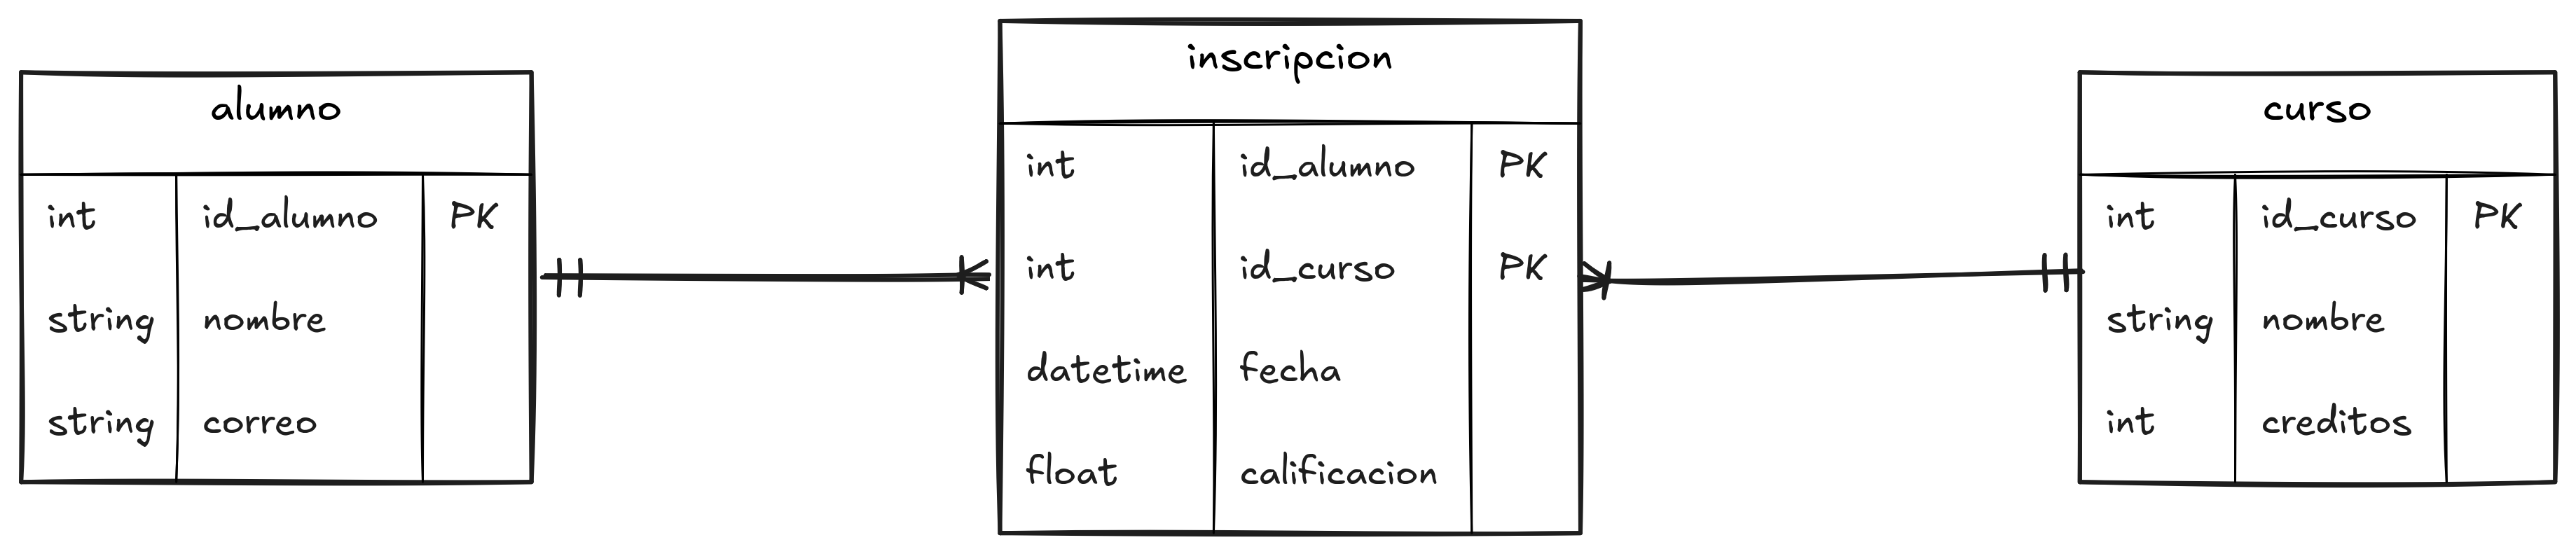
\includegraphics[width=1\textwidth]{img/asignaciones.excalidraw.png}
	\caption{Asignaciones}
    \label{fig:asignaciones}
\end{figure}

\begin{figure}[htb]
	\centering
	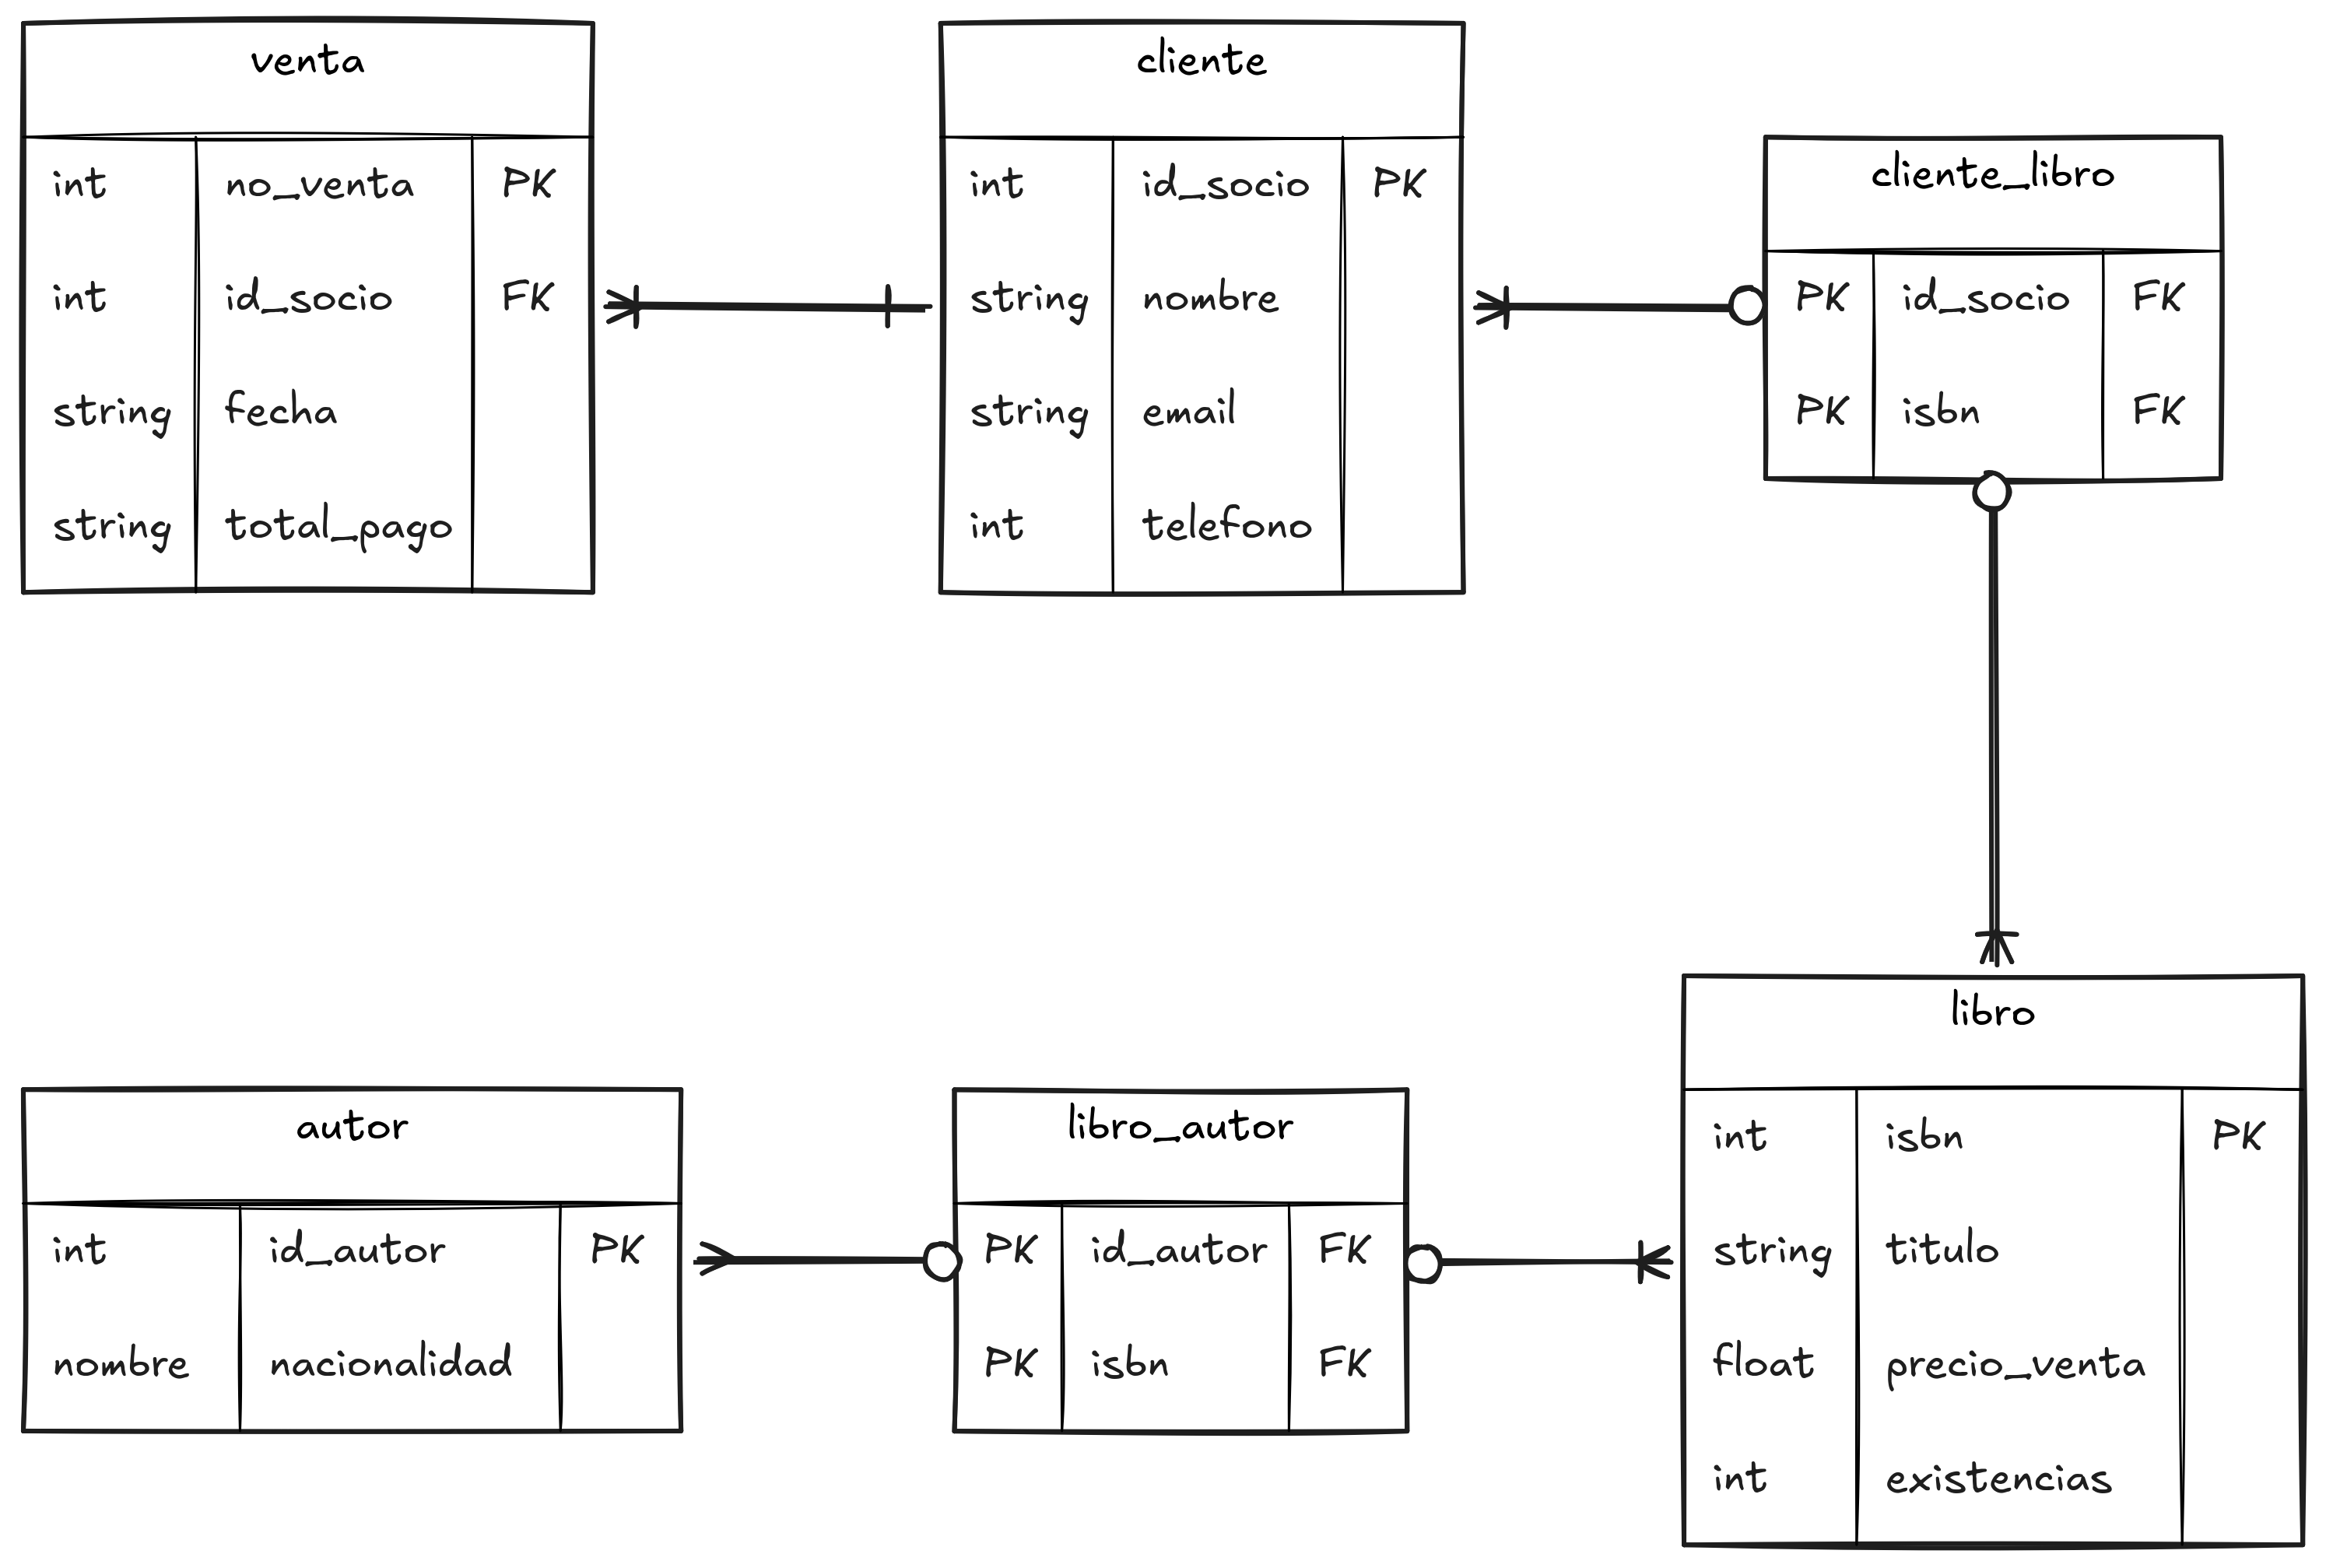
\includegraphics[width=1\textwidth]{img/libreria.excalidraw.png}
	\caption{Librería \textquote{El Párrafo}}
    \label{fig:libreria}
\end{figure}

\end{document}